\documentclass{article}
\usepackage[utf8x]{inputenc}
\usepackage[a4paper, margin=1in]{geometry}
\usepackage{enumitem}
\usepackage{xfrac}
\usepackage{lmodern}
\usepackage{amsmath,amssymb}
\usepackage[]{pdfpages}
\usepackage{multicol}
\usepackage{gensymb}
\usepackage{textcomp}
\usepackage{caption}
\usepackage{graphicx}
\usepackage[colorlinks=true,linkcolor=black]{hyperref}
\usepackage{varwidth}
\usepackage{listings}
\usepackage[bottom]{footmisc}
\usepackage{cleveref}
\usepackage{fancyhdr}

\pagestyle{fancy}
\fancyhf{}
\lhead{Morfeas RPi Hat}
\chead{Technical Reference}
\rhead{Page \thepage}
\rfoot{Page \thepage}

%Title declaration
\title{\huge``Morfeas RPi Hat''\\Technical Reference}
\date{}
\author{}

\begin{document}
%Title page
\clearpage
\begin{figure}
\centering
	
\includegraphics[width=2.5in]{../../../Docs/Morfeas_project_Documentation/ArtWork/Morfeas_logo_cyan.png}
\end{figure}
\maketitle
\thispagestyle{empty}
\begin{figure}
\centering
	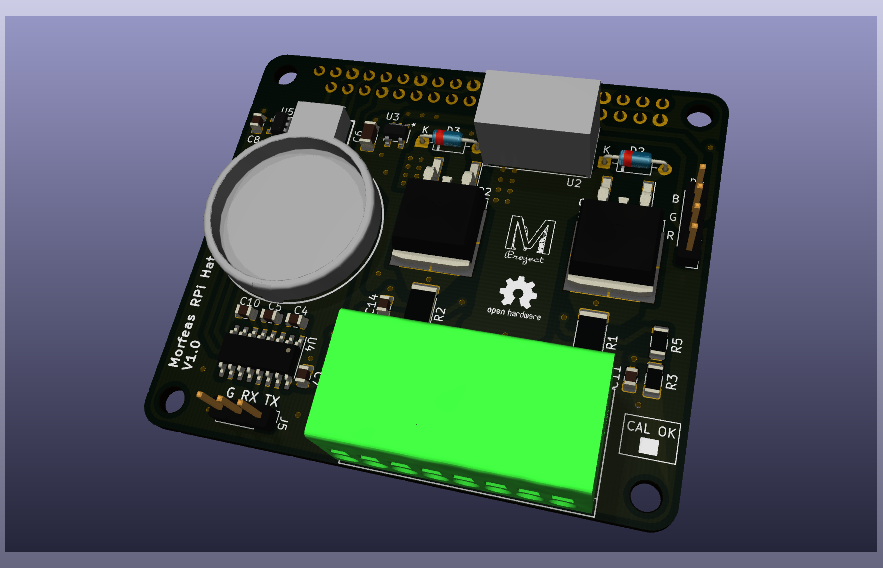
\includegraphics[width=3in]{./Artwork/PCB_3d_render.png}
\end{figure}
\newpage
%History page
\section{Change History}
Dec 7,12020 : Sam Harry Tzavaras -- Initial Work.
%License page
\newpage
\section{License}
Copyright (C)  12019  Sam Harry Tzavaras.\\
Permission is granted to copy, distribute and/or modify this document
under the terms of the GNU Free Documentation License, Version 1.3
or any later version published by the Free Software Foundation;
with no Invariant Sections, no Front-Cover Texts, and no Back-Cover Texts.
A copy of the license is included in the section entitled "GNU Free Documentation License".
\section{Disclaimers}
The following document referred as Technical Reference of the Morfeas RPI hat. Thus, evolving description of hardware. Any modification of it must take as responsibility of
the technician which did it. The author of this document does not have any responsible for any damage that this device can make after or before of any kind of modification. 

\section{Introduction}
The Morfeas project was initially start as an implementation of a software gateway solution system
(currently named Morfeas-Proto) that provide (and translate) measurements data from some proprietary devices (SDAQ family)
with CANbus compatible interface (SDAQnet) to OPC-UA protocol (Open62541).

As the Morfeas project developed additional support added for other devices (MDAQ, IO-BOX, MTI) with different interfaces (ModBus-TCP).

Furthermore, a web interface sub-project added to the Morfeas project under the name "Morfeas-web".
Thisof, will provide a layman friendly configuration interface for the gateway, the OPC-UA server's Nodeset and the connected devices.
\newpage
%Contents page
\newpage
\tableofcontents
\newpage
\section{Hardware Design}
\begin{figure}[h]
	\centering
	
\includegraphics[width=\linewidth,angle=0]{./Artwork/System.png}
	\caption{Morfeas RPI Hat's Block diagram}
	\label{fig:block}
\end{figure}

At figure~\ref{fig:block} present the design of the Morfeas RPI Hat in a simplified block diagram. The connection between the Raspberry PI and the Morfeas RPI hat done
from the RPi pin header that provided on the Raspberry board for expansion. From the pins that provided only the $I^2C$, UART, 5V power and some GPIO are used.
The 5V Power pins used to feedback with power the Raspberry Pi computer, for this a dedicated step down converter where is located onboard,
in addition the Power supply is supplying with power all the circuits that exist on board.

The UART pins driven directly to a dedicated LVTTL to RS-232 converter and from this directly a female pinhead. From there it's can be connected to any kind of connector
(like DB-9).

The $I^2C$ bus is the main communication way between the device onboard and the Raspberry pi computer. The device that communicating by this described bellow.
\begin{itemize}
	\item Current Sense Amplifier(CSA), one for each Port.
	\item Configuration serial EEPROM.
	\item Real Time Clock.
\end{itemize}

The CSAs are implemented my the MAX9611 which is a integrated circuit with main functionality to provide current measurements by reading the voltage of a shunt resistor on the high supple side.
In addition, the same IC can digitize the measurements of port's current, Output voltage and it's own temperature. All of them can be read by the $I^2C$ Bus.
Also the same IC can used as a electronic fuse in linear or switching mode. For the implementation of the Morfeas RPI Hat the MAX9611 ICs are configured to work in the switching mode.
The MAX9611 are controlling P-Channel MOSfets that are switching ON or OFF the power of the port.
The threshold point is programmed by two resistors that make a voltage divider. The threshold limit for each Channel is approximately 4 Amperes.\\
More information for this can be found at the MAX9611's Datasheet at the ``Datasheets" directory inside the ``Hardware" folder.

The Configuration EEPROM (24AA08) give or get the calibration table for each CSA on request of the Morfeas system, or the Morfeas\_RPI\_Hat software.
This EEPROM have four individual memory pages with 2kbit in each.
For the current implementation of the Morfeas RPI Hat only two of them are used to store the calibration tables.

The RTC is an IC that keeping track of the absolute time. In general provide the functionality on a computer to can have the absolute time in every request.
The RTCs must have a battery as second supply that will allow them to count even if the main supply is off power.
Some RTCs required to have an external crystal resonator where use as part of the feedback filter of Pierce oscillator.
The frequency of the oscillator is derived from the characteristics of the filter and because is crystal based it have very good stability ($\pm3.5ppm$).
The output of the oscillator is used as a clock signal for a programmable counter where is counting the time. The IC (DS3231) that have been chosen for this design have all the part of the oscillator (including the filter) integrated.\\
The communication with this IC done by $I^2C$ bus. All the operate with the RTC is handled by the kernel of the GNU operating system.

In addition to all the above the Morfeas RPI Hat using also some extra GPIO pins from the RPI Header that driving a RGB LED.
This have purpose to provide an indication of the mode of the Morfeas System (Morfeas\_SDAQ\_if).



\section{Software for Morfeas RPI Hat}
The supporting software for the Morfeas RPI hat is located under ``./src/Morfeas\_RPi\_Hat/" directory. This include the driver and the controlling software that used in calibration.
The subsection bellow will deal specifically with the controlling software that have name ``Morfeas\_RPi\_Hat".

\subsection{Installation of ``Morfeas\_RPi\_Hat"}
To compile the ``Morfeas\_RPi\_Hat" you need the following dependence:\\
* [GCC] - The GNU Compilers Collection\\
* [GNU Make] - GNU make utility\\
* [NCURSES] - A free (libre) software emulation library of curses.\\
* [GLib] - GNOME core application building blocks libraries.\\
* [LibGTop] - A library to get system specific data.\\
* [libi2c] - A library that provide I2C functionality to Userspace\\

The ``Morfeas\_RPi\_Hat" can be compiled and install from source by following the instruction of README.md file where located on the same directory with the source of the program.

\subsection{Usage}
The ``Morfeas\_RPi\_Hat" after it's installation can be called from bash by it's name. At listing~\ref{lst:usage} the help of it is presented.\\
The options `-b' used to redirect to an another $I^2C$ Bus.

The ``Morfeas\_RPi\_Hat" using curses to implement it's user interface. At figure~\ref{fig:Morfeas_RPi_Hat_UIF} a view of it is presented.\\
The user's interface is split in to two sections, the upper section with the readings and the lower with the Shell. 
The upper section is also spited in to up to four windows, one for each SCA(Even if the Morfeas RPi Hat shield support only two CSA the controlling software is make to be future proof).
The information that present on each window are: Name of the Port, Date of last calibration, current port's voltage, amperage and temperature of the shunt(in reality of the chip where is close to the shunt resistor).\\

The lower part of user interface is the shell which the user can enter commands. The command set is present on the usage of the program and also can be recall with the press of the question mark(?).  

The command are:    
\begin{itemize}
	\item \textbf{meas p\#}: Print the current measurements of CSA.
	\item \textbf{config p\#}: Read the EEPROM and print the port's configuration.
	\item \textbf{set p\# (czero,vzero,vgain,cgain)}: Set the specified configuration parameter.
	\item \textbf{save p\#}: Save the current Port's configuration in to EEPROM. 
\end{itemize}
All the commands called for a specific port. This done by the giver `p' followed by a number where represent the number of the port (aka 0..3).
\newpage
\begin{lstlisting}[frame=single,caption=Usage of ``Morfeas\_RPi\_Hat", label=lst:usage]
Usage: Morfeas_RPi_Hat [Options]
    Options:
             -h : Print Help
             -v : Print Version
             -b : I2C Bus number (default 1)

        -----Morfeas_RPi_Hat Shell-----
KEYS:
    KEY_UP    = Buffer up
    KEY_DOWN  = Buffer Down
    KEY_LEFT  = Cursor move left by 1
    KEY_RIGTH = Cursor move Right by 1
    Ctrl + C  = Clear current buffer
    Ctrl + L  = Clear screen
    Ctrl + I  = print used CAN-if
    Ctrl + Q  = Quit
COMMANDS:
    meas p# = Print measurement of Port's CSA
    config p# = Print Port's Configuration
    set p# czero = Set port's current zero offset
    set p# vzero = Set port's voltage zero offset
    set p# vgain Ref_value = Calculate and set CSA's voltage gain
    set p# cgain Ref_value = Calculate and set CSA's current gain
    save p# = Save Port's configuration to EEPROM
\end{lstlisting}

\begin{figure}[h]
\centering
	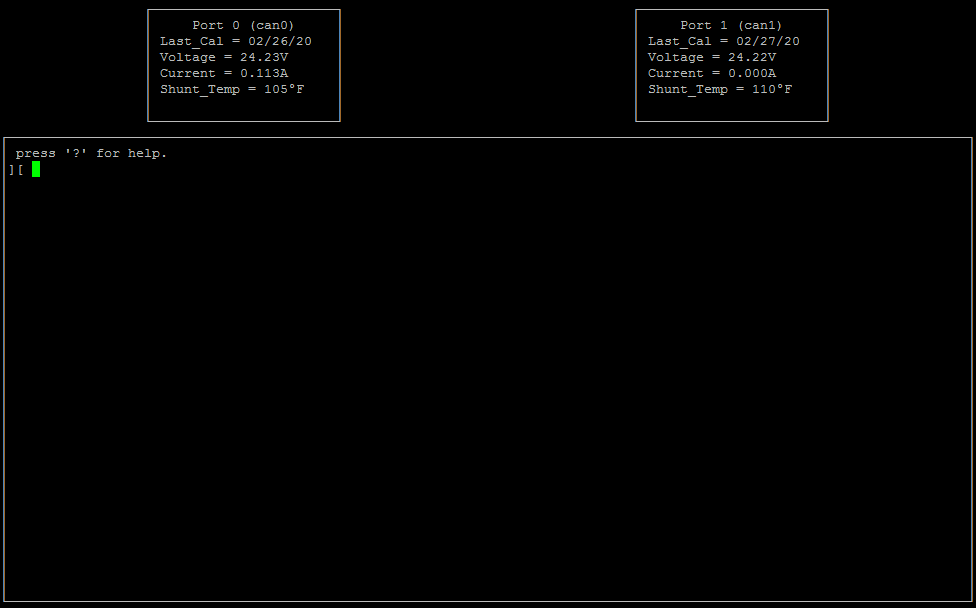
\includegraphics[width=5in,angle=0]{./Artwork/UIF.png}
	\caption{User interface of ``Morfeas RPI Hat"}
	\label{fig:Morfeas_RPi_Hat_UIF}
\end{figure}
\newpage
\section{Calibration}
\subsection{Required}
For the calibration procedure it's required some kind of resistive load that will load the port's power out. This can be done from a device as it's show at figure~\ref{fig:calibrator_top}.
\begin{figure}[h!]
	\centering
	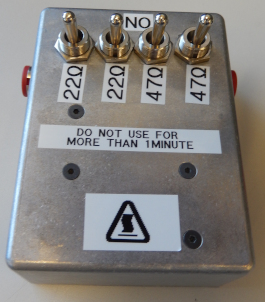
\includegraphics[width=2.5in]{./pics/calibrator_top.jpg}
	\caption{Top view of the Calibrator device}
	\label{fig:calibrator_top}
\end{figure}
The calibration device it's have inside some resistors and some sampling points for the measurements of voltage and current. At figure~\ref{fig:calibrator_block} is shown a cartoon type diagram
of the calibrator device.
\begin{figure}[h!]
	\centering
	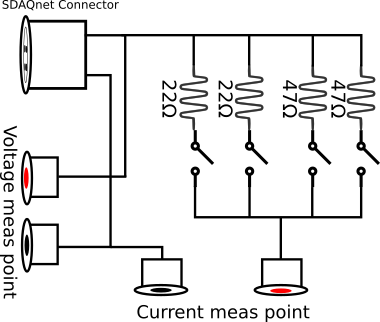
\includegraphics[width=3in]{./Artwork/calibrator_block.png}
	\caption{Calibrator's BLock Diagram}
	\label{fig:calibrator_block}
\end{figure}

For the calibration procedure are required:
\begin{itemize}
	\item The calibration device.
	\item One DMM configured as voltmeter.
	\item One DMM configured as Ammeter.
	\item Banana terminal cables.
	\item A short($\leq10''$) 4pin Lemo cable
\end{itemize}
\newpage
\subsection{Calibration Procedure}
The calibration procedure start by booting the computer that runs the Morfeas system and after finishing of boot continue with a request of stop of the Morfeas system from the systemd.
Then continue by executing the ``Morfeas\_RPi\_Hat" software. Then connect the two DMMs on the calibrator device and the calibrator device to the first port of the computer that is equip with the Morfeas RPi Hat.
All the switches of the calibrator must be open.\\
The first command where is issued is ``set p\# czero" (with all the switches open). This will zero the offset error of the particular CSA. Then the value of voltage out of the channel that displayed
at the DMM is recorded. After of this issue ``set p\# vgain Rec\_Value". This will correct the reading of voltage. After of this calibration of current follow by apply some load to the port.
$3/4$ of the maximum value($4A$) is a good start. The value from the DMM that measure current is recorded and issued as correction with command ``set p\# cgain Rec\_value".
Load now can be removed. A Check for linearity can be done by comparing the readings of DMM and CSA in different load values. A $1\%$ error is the maximum allowed.
In case that this is not satisfied repeat the current calibration with a different load. Otherwise save the configuration with command ``save p\#" and continue by repeating the above for the next port.
After of the calibration finish place a bullet on the ``CAL OK" mark on the front of the PCB
***The ``\#" on the above must be replaced with the number of the Port.\\

All of the above briefly:
\begin{enumerate}
	\item Boot the computer.
	\item Issue stop of the Morfeas System.
	\item Connect DMMs on Calibrator.
	\item Open all switch of the calibrator.
	\item Connect Calibrator with the a port.\label{loop}
	\item Issue ``set p\# czero".
	\item Record the Voltage measurement from DMM.\label{voltage}
	\item Issue ``set p\# vgain Rec\_Value" with the previously recorded value.
	\item Compare measurement DMM with SCA. if error ($>5\%$) go to \ref{voltage} and repeat.
	\item Load the port.\label{current}
	\item Record Value of current from DMM.
	\item Issue ``set p\# cgain Rec\_value" with the previously recorded value.
	\item Check Linearity ($\leq1\%$) by comparing readings of DMM and CSA.\\ if not satisfied go to \ref{current} and repeat.
	\item Issue ``save p\#" to save the port's configuration to EEPROM.
	\item Go to \ref{loop} and repeat for next port.
	\item Mark ``CAL OK". 
	\item Issue Start of the Morfeas System.
	\item Done.
\end{enumerate}

\newpage
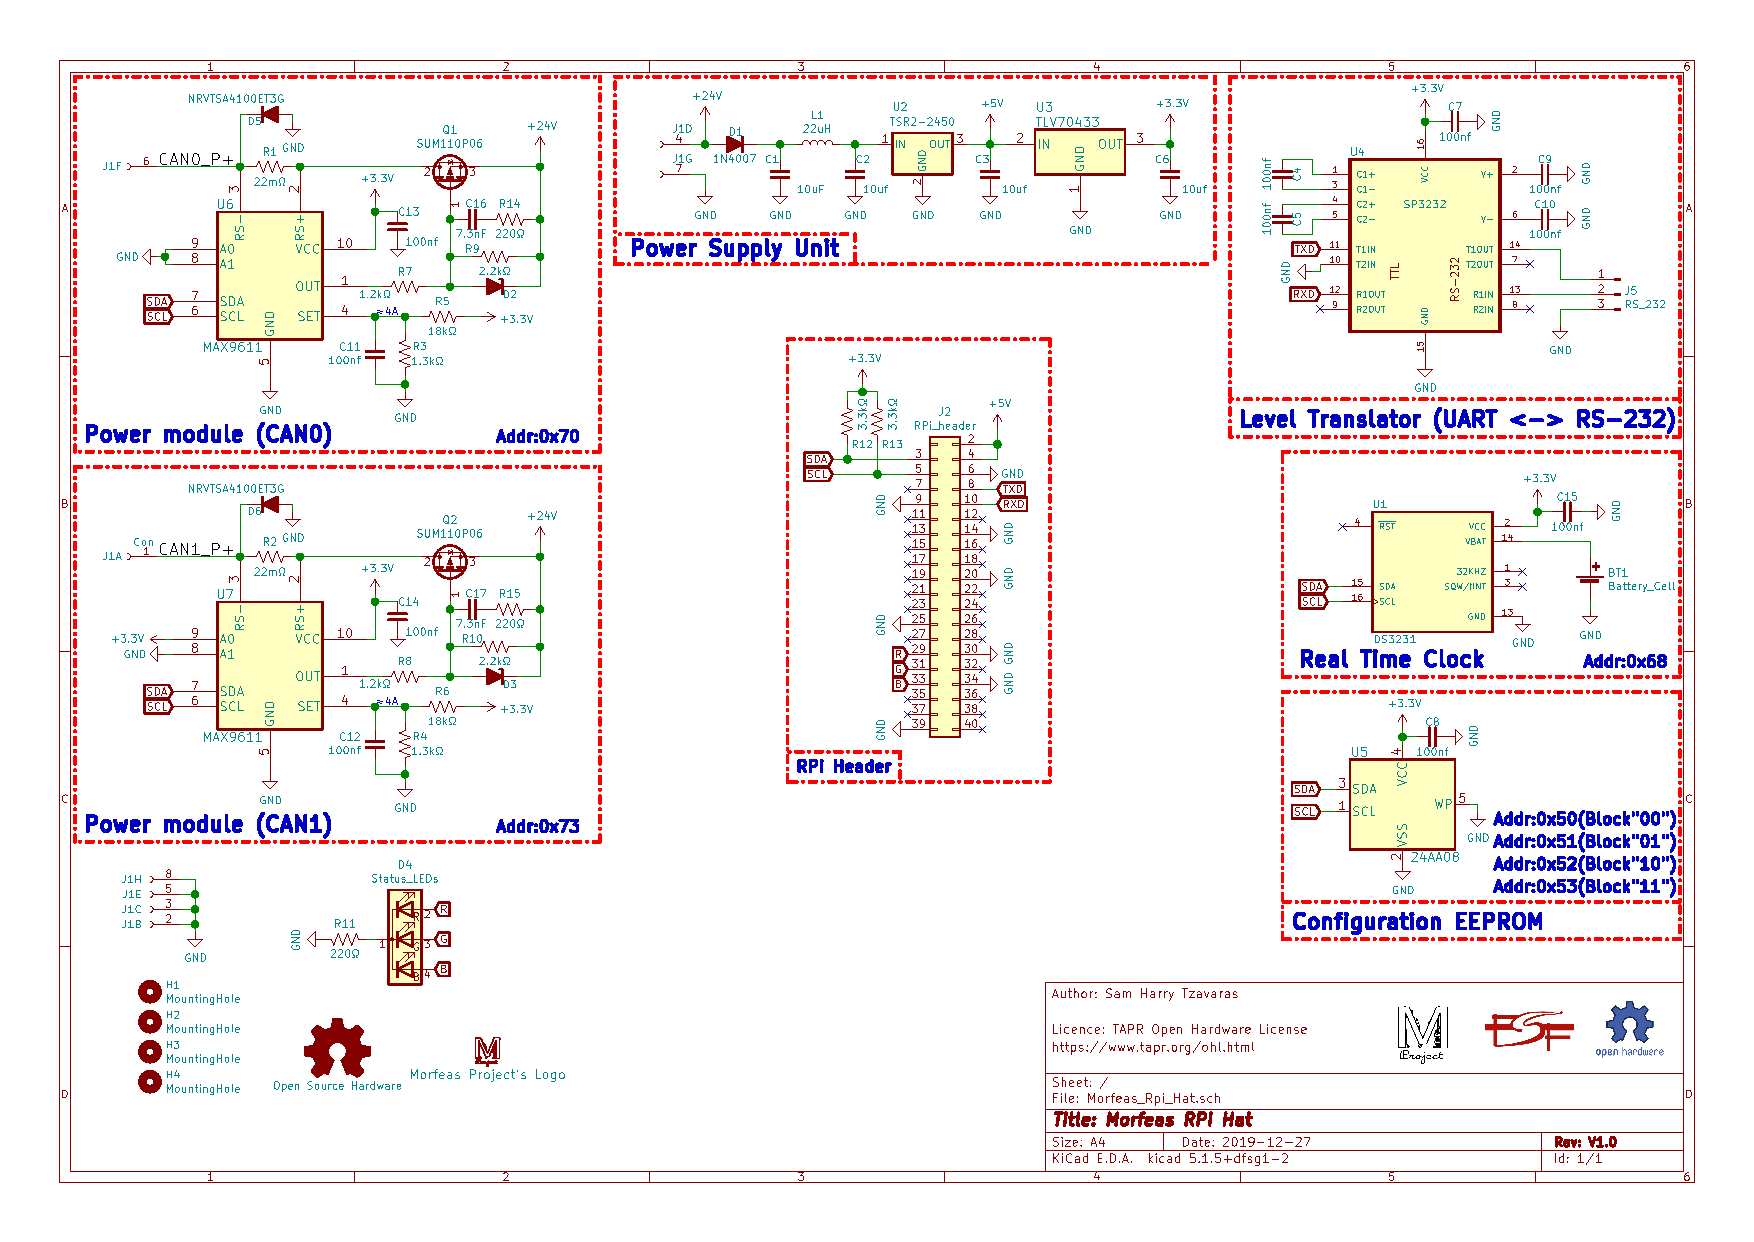
\includepdf[pages=-,scale=.85,offset=0in -.375in,pagecommand={\section{Appendix}\subsection{Morfeas RPI Hat Schematic diagram}},linktodoc=false,angle=-90]
{../Hardware/Exports/Morfeas_Rpi_Hat.pdf}
\newpage
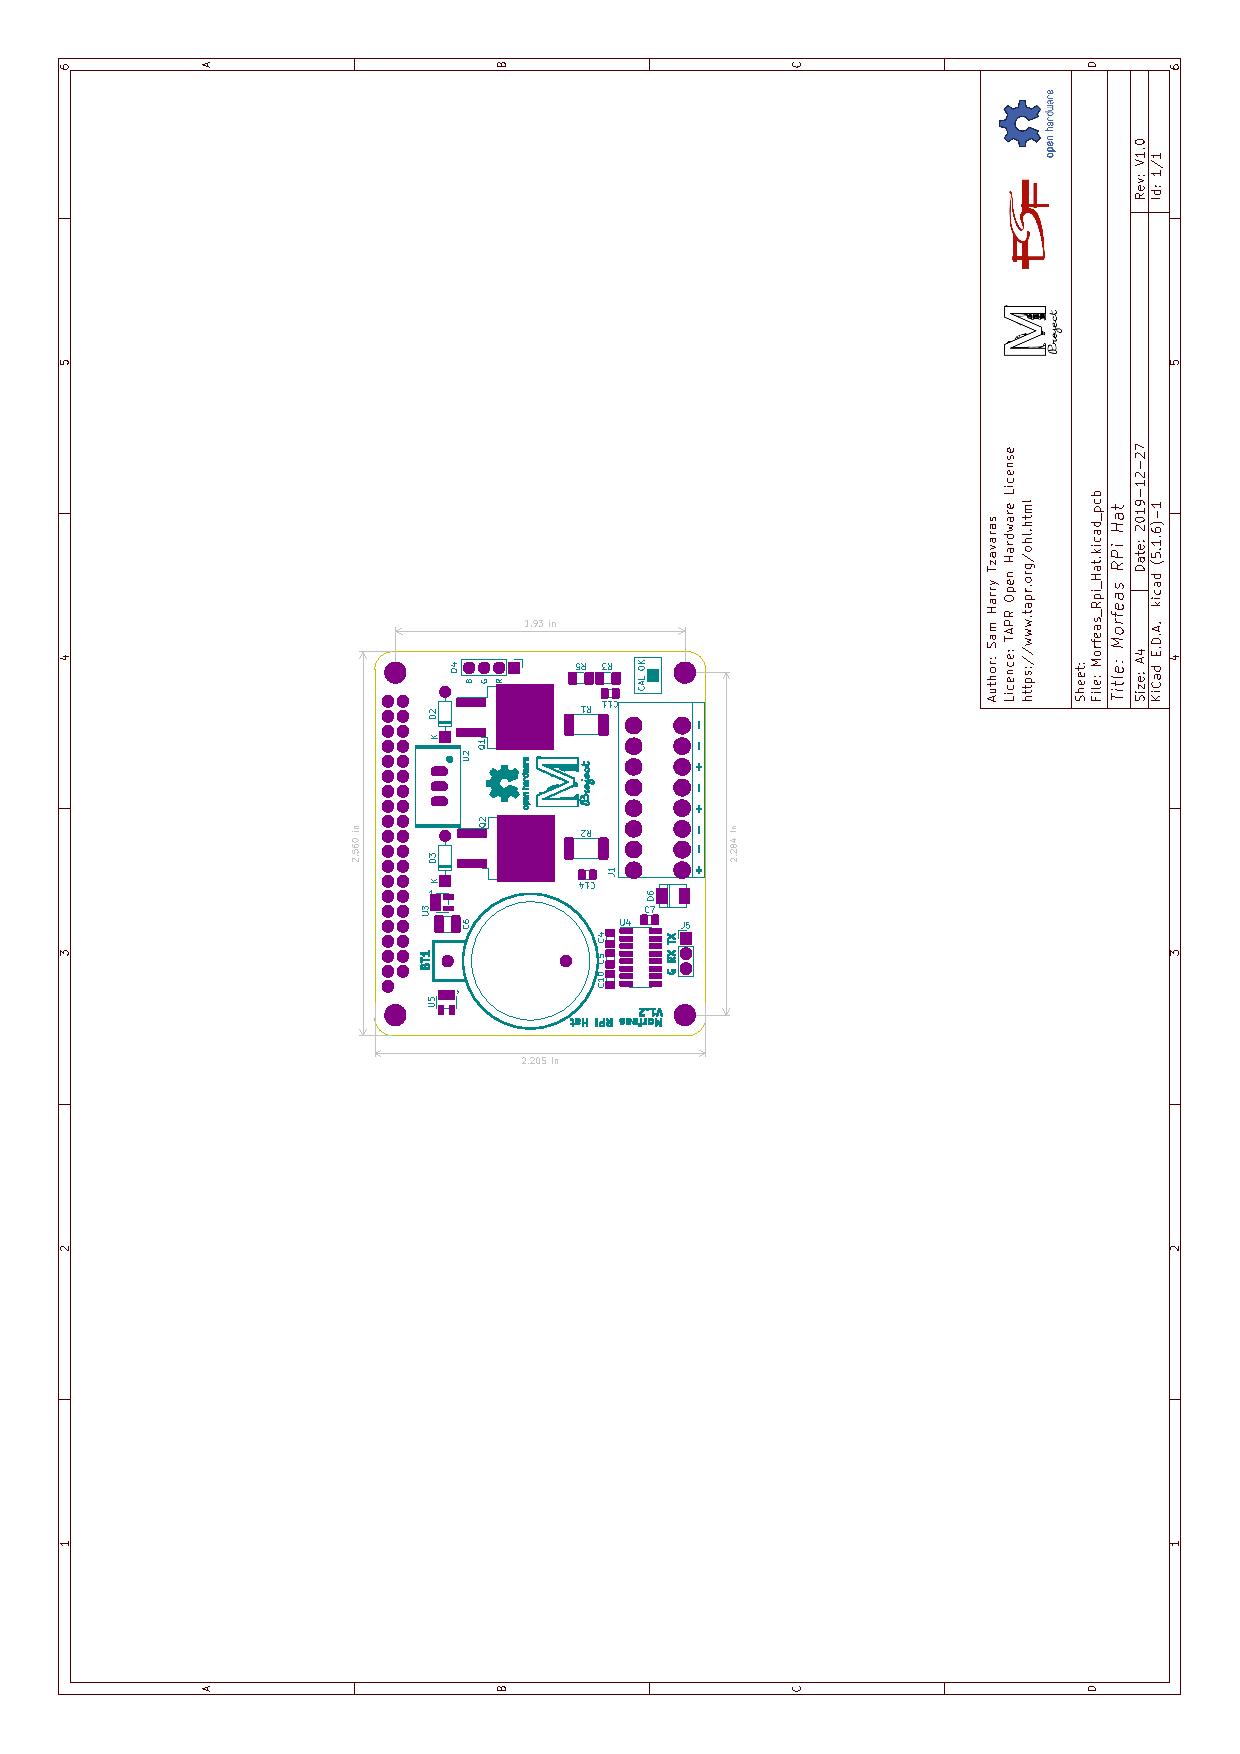
\includepdf[pages=-,scale=.89,offset=0in -.22in,pagecommand={\subsection{Morfeas RPI Hat Dimentions}},linktodoc=false,angle=-180]
{../Hardware/Exports/Morfeas_RPI_HAT_Dim.pdf}
\newpage
\subsection{Pictures}
\begin{figure}[ht]
\centering
	\includegraphics[width=\linewidth,angle=0]{./pics/PCB_side.jpg}
	\caption{Unpopulated PCB of Morfeas RPi Hat}
\end{figure}
\begin{figure}[ht]
\centering
	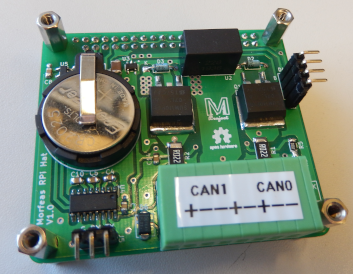
\includegraphics[angle=0]{./pics/Morfeas_RPi_HAT_top.png}
	\caption{Morfeas RPi Hat populated. Top view}
\end{figure}
\begin{figure}[ht]
\centering
	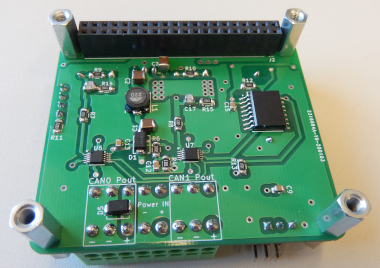
\includegraphics[angle=0]{./pics/Morfeas_RPi_HAT_bottom.png}
	\caption{Morfeas RPi Hat populated. Bottom view}
\end{figure}
\begin{figure}[ht]
\centering
	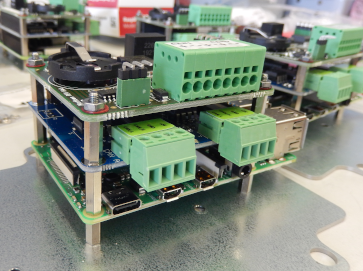
\includegraphics[angle=0]{./pics/Morfeas_stack.png}
	\caption{Computer stack in production}
\end{figure}
\end{document}

